\chapter{The LIGO detector}
\label{chapter2}
%\doublespace

\section{An interferometric gravitational wave detector}

The purpose of the LIGO detectors is to measure the faint
oscillations of spacetime imparted by far-away astrophysical
processes.  Through clever design and careful engineering, these
machines are capable of resolving these tiny perturbations from the
much louder sea of noise on the surface of the Earth\cite{Saulson1994Fundamentals}.

As we have seen, a passing gravitational wave modulates the optical
path length of light passing between inertial test
masses.  To exploit this effect and build a detector around it, we
need to arrange to have inertial test masses.  We need to be able to
tell the difference between phase perturbations due to the
gravitational wave and phase perturbations inflicted by our light
source.  We need to eliminate sources of phase variations that would
be louder than the effect we wish to measure.  

The essential points are:
\begin{itemize}
\item We approximate inertial test masses by hanging the optics as
  pendula.  These act as inertial masses above the pendulum resonance.
\item We build a Michelson interferometer for its common-mode noise
  rejection.  This is nicely compatible with the tensor action of
  gravitational waves.
\item To enhance the effect from a passing gravitational wave, we make
  the arms as long as possible.  To further enhance the response, we
  have the light travel this path many times, by using resonant cavities.
\item To increase the optical response to a gravitational wave, we
  increase the light power in the interferometer by using power
  recycling.
\end{itemize}
The following sections describe these principles in further detail.
\section{the Michelson interferometer}
\begin{figure}
\centering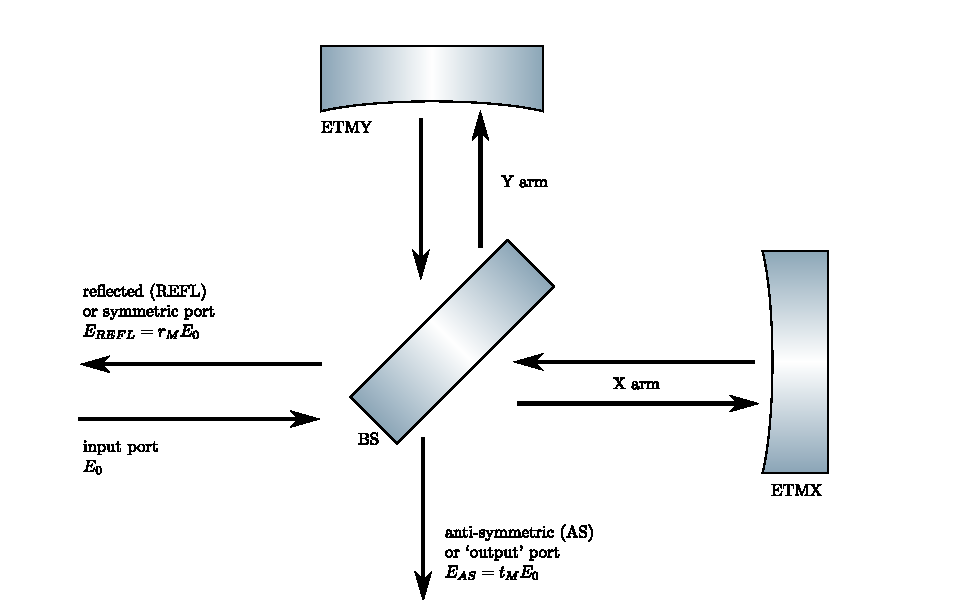
\includegraphics{figures/michelson.pdf}
\caption[Michelson interferometer]{\label{fig:michelson}Michelson
  interferometer.  This figure introduces some of the common
  nomenclature for the ports and optics of the Michelson
  interferometer.  ETM stands for `end test mass.'}
\end{figure}

Contemplating the effect of a gravitational wave on a ring of test
particles (figure~\ref{fig:gwave-effect}), it is easy to imagine
constructing a Michelson interferometer (figure~\ref{fig:michelson})
with its beamsplitter in the center of the circle and with two of the
test particles forming the end mirrors of the Michelson.  More
importantly, the Michelson allows us to separate the differential
motion of the two arms from the common motion, which is
indistinguishable from laser frequency changes.

If we assume a perfect (lossless, 50/50) beamsplitter, the
transmission and reflection coefficients for the Michelson are:
%
\begin{align}
t_M  &= \frac{1}{2}\left(r_x \exp \{i2\phi_x\} - r_y \exp\{i2\phi_y\} \right) \\
r_M  &= \frac{1}{2}\left(r_x \exp \{i2\phi_x\} + r_y \exp\{i2\phi_y\} \right)
\end{align}
where $r_{\{x,y\}}$ are the amplitude reflectivities of the x- and y-arm mirrors, and $\phi_{\{x,y\}}$ are 
the phases accumulated as the light travels from the beamsplitter to end mirrors.  It is useful to change
our variables to express these quantities in terms of the differential and common reflectivies and phases.
Making the substitutions
\begin{align}
\phi_- &= \phi_x - \phi_y       &  \phi_x &= \phi_+ + (1/2)\phi_- \\
\phi_+ &= (\phi_x + \phi_y)/2   &  \phi_y &= \phi_+ - (1/2)\phi_-
\end{align}
and
\begin{align}
  \Delta r & = r_x - r_y        &  r_x   &= r + (1/2)\Delta r \\
       r & = (r_x + r_y)/2      &  r_y   &= r - (1/2)\Delta r
\end{align}
yields
\begin{align}
t_M  &= e^{i2\phi_+} \left( i r\sin \phi_- + (\Delta r/2) \cos \phi_- \right) 
\label{eq:michelson-transmission}\\
r_M  &= e^{i2\phi_+} \left( i r \cos \phi_- + (\Delta r/2) \sin \phi_- \right) 
\end{align}

The intent is for the arm reflectivities to be identical (so $\Delta r \to
0$), and to operate near the \emph{dark fringe} ($\phi_-\to0$) so that
the input field does not couple directly to the output port
(i.e. $t_M\to0$).  Given this configuration, there are two salient
points concerning gravitational wave detection:
%
\begin{itemize}
\item Variations of the differential phase $\phi_-$ \emph{linearly couple} to the \emph{field amplitude} at the output port.
\item Variations of the common phase $\phi_+$ do not couple.
\end{itemize}
%
The field at the output port will thus be sensitive to suitably
polarized graviational waves but insensitive to laser frequency noise.
(An orthogonally polarized gravitational wave, whose strain ellipse is
rotated $45^\circ$, will modulate $\phi_+$ but this detector
sacrifices sensitivity to that polarization in order to gain
common-mode noise immunity.)  

Ultimately, we can not measure optical field amplitudes directly, but
only the power, i.e. the envelope of the optical field, as the field
itself oscillates at at $c/(1064\text{ nm})\approx 300\text{ THz}$,
much too quickly to measure directly.  We compute the power at the
anti-symmetric and reflected ports by taking the squared magnitude of
the field amplitudes.  Using $P_{AS} = P_{BS} \left|t_M\right|^2$ and
$P_{REFL} = P_{BS} \left|r_M\right|^2$:
%
\begin{align}
P_{AS}   &=  P_{BS}\left( {r}^2 \sin^2 \phi_- + (\Delta r/2)^2 \cos^2 \phi_-\right) \\
P_{REFL} &=  P_{BS}\left( {r}^2 \cos^2 \phi_- + (\Delta r/2)^2 \sin^2 \phi_-\right) 
\end{align}

The power transmitted through the Michelson at the dark fringe is the
\emph{contrast defect},
%
\begin{equation}
c_d = \frac{P_{AS}}{P_{BS}} = \frac{1}{4}\left(\Delta r\right)^2.
\end{equation}

The linear relationship between $\phi_-$ and the electric field at the
output port has turned into a quadratic relationship between $\phi_-$
and the output port power.  We will turn to the task of recovering a
linear signal in section~\ref{sec:isc}, but first we will consider
methods to magnify the effect of a gravitational wave on $\phi_-$.

\section{Resonant cavities}

One approach to increasing the phase imparted by the GW to the light
in the arms of the interferometer would be to arrange for the light to
make multiple traversals of the arm length.  This could be in the form
of a delay line (where the optical path makes several zig-zags down
the arm length in a definite number of bounces), or a resonant cavity
(made by facing two partially-transmissive mirrors at each other,
resulting in an effective number of bounces).  Resonant cavities were
chosen for the LIGO arms. 

The basic setup of a Fabry-Perot cavity is shown in Figure~\ref{fig:fabry-perot}.
Light entering the cavity will interfere with light already
circulating in the cavity.  If, after making a round-trip through the
interior of the cavity, the circulating light returns to its original
phase (and spatial distribution), constructive interference will occur
and the light will resonate in the cavity.  If the mirrors have high
reflectivity, then the light inside the cavity will survive for many
round-trips inside the cavity. Any deviation from the required $2\pi$
radians of round-trip phase will be magnified on each bounce.

The theory of the Fabry-Perot cavity is derived in 
appendix~\ref{sec:cavities}.  For the purpose of this chapter, we
need only the fact that changing the intra-cavity phase results in a
much greater change in the phase of the light reflected from the
cavity; the ratio of these phase changes is the \emph{phase gain},
given by $g_\phi = r_c'/r_c$, where $r_c$ is the cavity reflectivity on
resonance, and $r_c'$ is its derivative with respect to changes in
intra-cavity phase.  The numerical values for $r_c$ and $r_c'$ in terms of the individual mirror reflectivities (for a lossless cavity) are (as derived in appendix~\ref{sec:cavities} or given in \cite{LigoFreqResponse97}):
%
\begin{align}
r_c & = \frac{r_1 - r_2}{1 - r_1 r_2} &
r_c'& = \frac{\left(1 - {r_1}^2\right)r_2}{\left(1 - r_1 r_2\right)^2}
\end{align}

% FIXME: Should mention the idea of the cavity averaging the field.

% FIXED Gaby says: You should mention this is a frequency dependent gain,
% and explain the long wavelength appoximation.

\label{sec:long-wavelength}We typically work in the \emph{long wavelength approximation}, in
which we assume that the gravitational wave strain (or cavity length)
changes slowly compared to the time required by light to travel from
one mirror of the cavity to the other.  Because light and
gravitational waves travel at the same speed, this requires that the
GW wavelength be much longer than the interferometer arm length.  
%(At higher frequencies, the response of the interferometer is modified;
% this is discussed in appendix~\ref{sec:antenna-pattern}.)

\section{Michelson with Fabry-Perot arms}

By replacing the end mirrors of our Michelson interferometer with
Fabry-Perot cavities, the sensitivity to phase differences increases
by a factor of the phase gain.  

We now have
\begin{equation}
t_M  = e^{i 2 g_\phi \phi_+} 
\left( r_c i \sin g_\phi \phi_- + 
        \frac{\Delta r}{2} \cos g_\phi \phi_- \right)
\end{equation}
where $\Delta r$ now gives the difference between the reflectivites of the
two arm \emph{cavities}.

For Enhanced LIGO, the phase gain is approximately 140.

\section{Power recycling}

The Michelson interferometer tuned to a dark fringe for the laser
carrier sends most of the laser power back towards the laser.  Instead
of discarding this power, it can be sent back into the Faby-Perot
Michelson interferometer.  This is done by adding an additional
mirror, the \emph{power recycling mirror}, that forms a resonant
cavity with the rest of the interferometer.  Choosing the reflectivity
of the power recycling mirror to match the effective reflectivity of
the rest of the interferometer makes this cavity critically coupled;
ideally all of the laser carrier is coupled into the interferometer
and very little is reflected.  Most of the light stays in the
interferometer until it is lost to scattering or absorption.

\section{The coupled cavity pole}

\begin{figure}
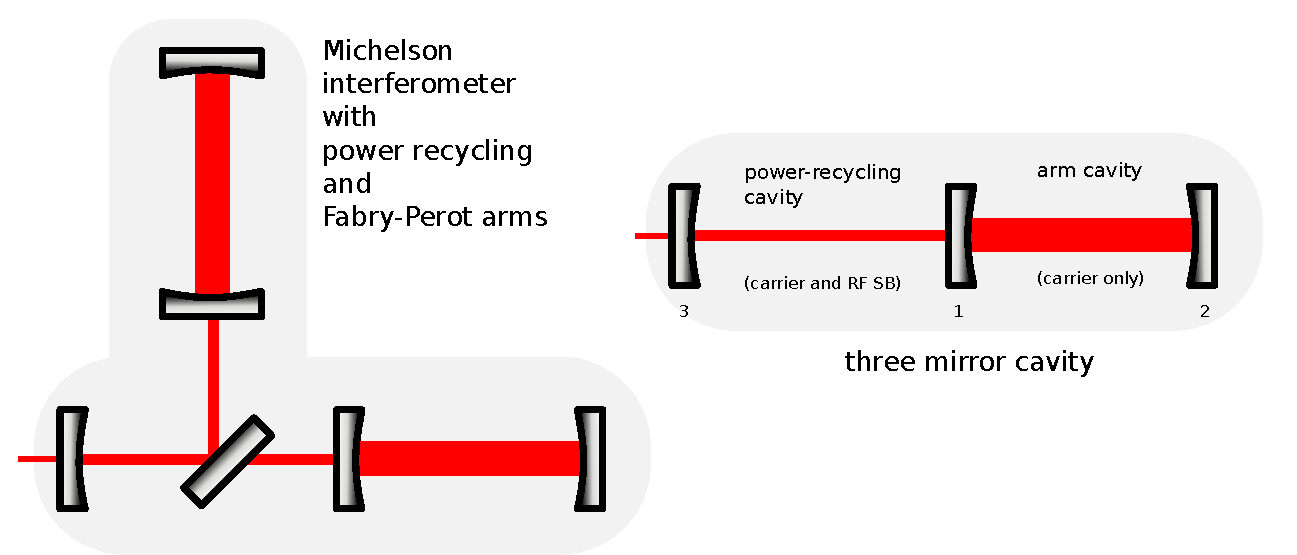
\includegraphics[width=\columnwidth]{figures/three-mirror-cavity.pdf}
\caption[Three mirror cavity]{It is sometimes convenient to condense the
two arms of the Power-Recycled Fabry-Perot Michelson interferometer into
a single `virtual arm' for the purpose of analysis.
\label{fig:three-mirror-cavity}}
\end{figure}

\begin{figure}
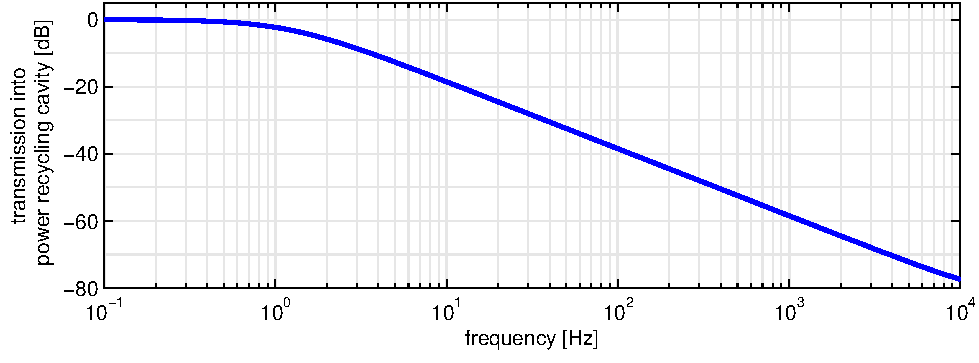
\includegraphics[width=\columnwidth]{figures/ccpole.pdf}
\caption[The coupled-cavity pole]{Transfer function from laser intensity
fluctuations incident on the interferometer to laser intensity fluctuations
inside the power recycling cavity.  Fluctuations around the laser carrier
above the coupled-cavity pole are attenuated.\label{fig:cctf}}
\end{figure}

The combination of the arm cavities and the power recycling cavity acts
in some ways like a single cavity with a much longer storage time than
either the arms or the PRC individually.  This produces a filtering 
effect that will prove essential when we discuss DC readout later on.

Because the two arm cavities are made to be as nearly identical as
possible, and because the Michelson is operated very close to the dark
fringe, we can condense the two arm cavities into a single cavity for
the purpose of analysis (depicted in figure~\ref{fig:three-mirror-cavity}.  
In considering the effect of amplitude or frequency perturbations of the 
input field, the power-recycled Fabry-Perot Michelson can be considered 
as a three mirror cavity.

It is useful to regard the cavity as acting as a linear operator on
the input fields.  To find the transfer function of the coupled
cavity, we can simply substitute the cavity reflectivity function
$r_c(\phi)$ given in equation~\ref{eq:cavity-reflectivity} into
itself, with suitable substitutions.
%
When this is done, it is found that the transfer function from fields at
the interferometer input to the field just inside the PRC can be well
described by a single pole at low frequency, the coupled cavity pole.
%
There is no closed-form solution for the exact value of the coupled-cavity
pole\cite{Rakhmanov2000Dynamics}, but a very good approximation 
results if we first compute the reflectivity of the shorter cavity on
resonance, and substitute this into the expression for the cavity pole
of the larger cavity. Doing this, we find
%
\begin{equation}
f_{cc} \approx \frac{1}{2\pi} \nu_0  \log \left(\frac{r_3 - r_1}{1 - r_1 r_3} r_2\right)
\end{equation}
where $f_{cc}$ is the frequency of the coupled cavity pole, $\nu_0$ is
the free spectral range of the arm cavity, and $r_{\{1,2,3\}}$ are the
reflectivities of the ITMs, ETMs, and recycling mirror, respectively.

The coupled cavity pole in Initial/Enhanced LIGO is approximately 1
Hz.  Astoundingly, this means that any amplitude or phase noise around
the laser carrier (itself oscillating at 300 THz!) will be attenuated
by $1/f$ above 1 Hz (see figure~\ref{fig:cctf}), making the carrier
light circulating in the interferometer some of the `quietest' light
available anywhere.  One of the motivations of DC Readout (chapter 5)
is to exploit this effect fully.  

% By comparison, the RF sidebands are resonant only in the PRC and not
% the arms, so they are affected by the coupled cavity pole.

\section{Interferometer Sensing and Control}
\label{sec:isc}

The power-recycled, Fabry-Perot Michelson optical configuration
(collectively referred to as ``the interferometer'') described above
exhibits the desired sensitivity to gravitational waves and immunity
to common mode noise.  However, it only does so when the Fabry-Perot
cavities are held on resonance, and the Michelson is held to the dark
fringe.  The need to sense the state of the interferometer and to use
feedback control to keep it at the desired operating point is known as
\emph{interferometer sensing and control} (ISC).  The initial LIGO
sensing and control scheme is described in~\cite{Fritschel2001Readout}
and \cite{Regehr1994Signal}.  A pedagogical introduction is provided
in \cite{Black2003Introduction}.

The \emph{control} aspect has not yet been mentioned.  To allow
actuation on the optics, the test masses are each equipped with five
small magnets (four on the face and one on the side) which fit into
solenoids mounted to the suspension structure.  This electromagnetic
drive allows forces to be exerted on the optics to control their
position and orientation.
 
%\section{Heterodyne detection}
The initial LIGO detectors were designed to use, as much as possible,
proven technologies.  The proven technique for sensing the
length/frequency mismatch of an optical cavity was the
Pound-Drever-Hall (PDH)
technique\cite{Drever1983Laser,Black2001Introduction}, sometimes
called reflection-locking, which can be used to lock the frequency of
a laser to the length of a cavity, or vice versa.

\begin{figure}
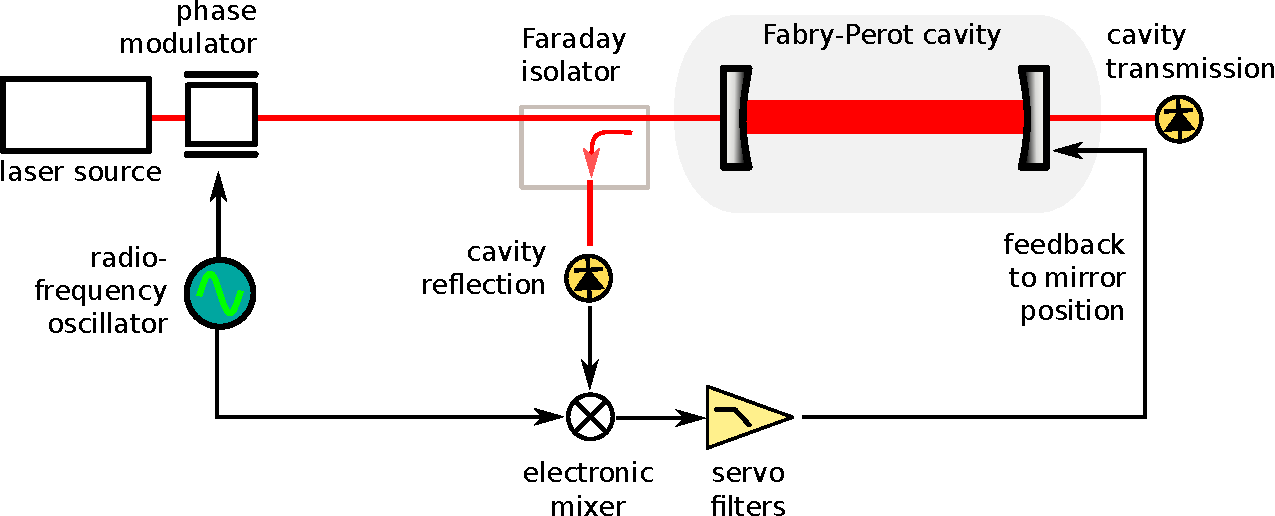
\includegraphics[width=\columnwidth]{figures/pdh-diagram.pdf}
\caption[Pound-Drever-Hall setup]{\label{fig:pdh-diagram}In the basic
Pound-Drever-Hall setup, a phase modulator is used to produce RF sidebands well 
outside of the cavity bandwidth.  The light reflected from the cavity
is incident on a photodiode, the signal from which is demodulated to
produce an error signal indicating the mismatch between cavity length
and laser carrier frequency.  Through feedback, the cavity can be `locked' 
to the resonance.  The technique can be generalized to sense and control
much more complex interferometers.}
\end{figure}

\begin{figure}
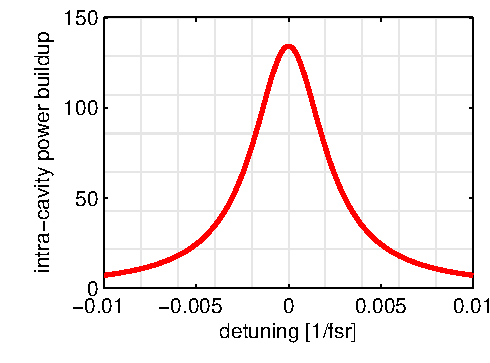
\includegraphics[width=0.5\columnwidth]{figures/cav-power.pdf}
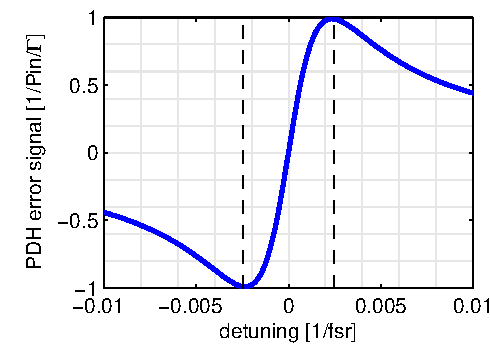
\includegraphics[width=0.5\columnwidth]{figures/cav-pdh.pdf}
\caption[Pound-Drever-Hall error signal]{\label{fig:pdh-error}
(a) Power buildup inside a resonant cavity relative to the incident
power, as a function of cavity detuning (deviation from resonance).
(b) The Pound-Drever-Hall error signal as as a function of detuning
(in watts relative to the incident power and the modulation depth).
The dashed lines indicate the region in which PDH provides a usable
error signal with which to lock the cavity.  The cavity modeled here
has parameters similar to the initial LIGO arm cavities.
}
\end{figure}

\subsection{The Pound-Drever-Hall technique}
In the basic PDH setup, the laser light incident on a resonant cavity
is first phase-modulated at a frequency well outside of the bandwidth
of the cavity, such that the sidebands are nearly anti-resonant in the
cavity when the carrier is resonant.  For small perturbations (in
laser frequency or cavity length) around this point, the phase of the
reflected carrier changes quickly, while the phase of the reflected
sideband field changes more slowly.  The reflected sideband field may
therefore be used as a local oscillator by which to measure the
carrier phase.

The phase modulation may be expanded in terms of sidebands using the
Jacobi-Anger expansion (see section~\ref{sec:jacobi-anger}):
%
\begin{align}
\exp\left\{i\Gamma\cos\Omega t\right\} 
  &= \sum_{n=-\infty}^{\infty} \left(i^n\right)  J_n(\Gamma) \exp\{i n \Omega t\} \\
  &= J_0(\Gamma) + i J_{1}(\Gamma) e^{i\Omega t} - i J_{-1}(\Gamma) e^{i -\Omega t}+\cdots %\\
%  &= J_0(\Gamma) + i J_{1}(\Gamma) e^{i\Omega t} + i J_{1}(\Gamma) e^{i \Omega t}+\cdots\\
%  &= J_0 + 2 i J_{1} \cos \Omega t + \cdots
\end{align}
From this expansion we see that phase modulation at a frequency
$\Omega$ results in the creation of an infinite number of sidebands
around the laser carrier, spaced at multiples of $\Omega$, and whose
amplitudes are given by the Bessel functions.  The magnitude of the
modulation ($\Gamma$, in radians) is known as the \emph{modulation
depth}.  We typically use a small modulation depth, so that only the
first-order sidebands are significant.  These first-order sidebands
are displaced from the carrier by the modulation frequency $\pm\Omega$
and have amplitude $J_1(\Gamma)$.

Upon reflection from a cavity the phases of the carrier and the two
sidebands will be rotated.  This phase rotation converts the phase
modulation to amplitude modulation, which is observed by the
photodiode.  Typically, the laser frequency or the cavity length is
adjusted to hold the carrier on resonance.  Near the resonance, there
is a very large change in reflected phase for a small change of
detuning (change in cavity length or laser frequency); the RF
sidebands, on the other hand, are typically far from resonance and
experience very little phase change.  As a result, a small perturbation
from resonance will turn the cavity into an FM-to-AM converter.  The
resulting amplitude modulation can be sensed by a photodiode and
demodulated to produce an error signal indicating how far the cavity
is from resonance.

\begin{comment}
The reflectivity of a lossless Fabry-Perot cavity is
\begin{equation}
r_c(\phi) = \frac{r_1 - r_2 \exp i2\phi}{1 - r_1 r_2 \exp i 2\phi}
\end{equation}
for an optical field that is $\phi$ radians from resonance.
The field reflected from the optical cavity is
%
\begin{equation}
E_r = \underbrace{E_0 e^{i\omega t}}_{\text{laser source}} \left(
\underbrace{J_0(\Gamma) r_c(\phi)}_{\text{carrier}}
+ 
\underbrace{\overbrace{i J_1(\Gamma) e^{-i\Omega t}}^{\text{incident field}}
            \overbrace{r_c(\phi - \Omega/\nu_0)}^{\text{cavity action}}}_{\text{lower sideband}}
+ 
\underbrace{i J_1(\Gamma) e^{ +i\Omega t} r_c(\phi + \Omega/\nu_0)}_{\text{upper sideband}}
\right)
\end{equation}
where $\phi$ now indicates the detuning of the carrier in the cavity
(i.e. its deviation from resonance) in radians, $\nu_0$ is the
cavity's free spectral range, and $\omega=2\pi c/\lambda$ is the
optical frequency.  Here we have assumed that higher order harmonics
($J_2(\Gamma)$, etc) are negligible.

A photodiode is sensitive only to power and not field amplitude; when
this field is incident on a photodiode, the photodiode will see the
squared magnitude of the field, i.e. $|E_r|^2 = {E_r}^* E_r$, where
$*$ indicates complex conjugation.  The interference of the carrier
and the sideband terms results in a DC (i.e. unchanging) power in
addition to power modulations at frequencies $\Omega$ and $2\Omega$.

\begin{align}
E = &E_0 + E_- e^{-i\Omega t} + E_+ e^{+i\Omega t} \\
P = & \left(E_0   + E_- e^{-i\Omega t} +  E_+ e^{+i\Omega t}\right)
      \left(E_0^* +   E_-* e^{+i\Omega t} + E_+^* e^{-i\Omega t}\right) \\
  = & |E_0|^2 + |E_-|^2 + |E_+|^2 \\
    & + E_0 E_+^* e^{-i\Omega t} + E_0^* E_- e^{-i\Omega t} \\
    & + E_0 E_-^* e^{+i\Omega t} + E_0^* E_+ e^{+i\Omega t} \\
    & + E_- E_+^* e^{-2i\Omega t} + E_-^* E_+ e^{+2i\Omega t} \\
  = & \\
    & + 2 \text{ Re } E_-^* E_+ e^{2i\Omega t}
\end{align}

\begin{equation}
\begin{split}
P_r = |E_0|^2 [ & {J_0}^2 |r_c(\phi)|^2 + {J_{-1}}^2  |r_c(\phi-\Omega/\nu_0)|^2 + {J_{1}}^2  |r_c(\phi+\Omega/\nu_0)|^2 + \\
             & \left(\right)e^{i\Omega t} \\
             & 2 {J_1}^2 \left(\text{Re } r_c(\phi-\Omega/\nu_0)^* r_c(\phi+\Omega/\nu_0)\right) \cos 2\Omega t
\end{split}
\end{equation}
\end{comment}

\subsection{Generalization of the PDH technique}

To sense and control the entire Power-Recycled, Fabry-Perot Michelson
interferometer, the PDH scheme can be generalized to sense all degrees
of freedom by providing one or more pairs of RF sidebands, and sensing
and demodulating the light at various interferometer ports.  In the
remainder of this dissertation, however, we are concerned only with
sensing the differential arm degree of freedom (DARM), which contains
the gravitational wave signal.

\begin{figure}
\includegraphics[width=\columnwidth]{figures/dc-readout-diagram.pdf}
\caption[Enhanced LIGO interferometer
  layout]{\label{fig:dc-readout-ifo}Enhanced LIGO interferometer
  layout (not to scale).  The dotted line represents the vacuum
  enclosure. The initial LIGO configuration is modified by adding an
  output mode cleaner and DC photodiodes.  A beamsplitter directs 97\%
  of the optical power to this new path and the remaining 3\% to the
  old RF heterodyne output chain, used for lock acquisition and
  automatic alignment.}
\end{figure}

\section{Noises}

No discussion of detector operation is complete without consideration of the
noises which limit detection.  The noise sources relevant to laser
interferometer gravitational wave detectors are articulated in Rai
Weiss's original design study\cite{Weiss1972Electromagnetically} and
Rana Adhikari's dissertation\cite{RanaThesis}.  It is often useful to
divide noises into \emph{displacement noises} (which correspond to
real displacement of the mirrors or intra-cavity phase modulation) and
\emph{sensing noises} (which arise in the sensing of the interferometer 
state).  Displacement noises include:

\begin{itemize}
\item \textbf{seismic noise} -- this refers to any motion of the mirrors due to
  local ground motion.  Below $\sim40$~Hz, the initial/enhanced LIGO
  noise floor is entirely limited by seismic noise (the so-called `seismic wall').
\item \textbf{thermal noise} -- thermally excited motion in the test mass
  suspensions and the high-reflectivity coatings produces displacement noise\cite{Saulson1990Thermal,Gonzalez1994Brownian},
  which currently limits the sensitivity in the range 40 - 100 Hz.
\item \textbf{quantum radiation pressure noise} -- the Poisson statistics of
  the light circulating in the arm cavities generates a white-noise
  random force, producing a $1/f^2$ displacement spectrum.  This noise
  source has not yet been observed, since its influence is masked by
  the other low-frequency noises.
\item \textbf{technical radiation pressure noise} -- variations in
  light intensity create varying radiation pressure forces.
\item \textbf{residual gas noise} -- any residual gas in the vacuum
  enclosure will displace the optics through Brownian motion, in addition to
  creating spurious phase modulation of the light.

\end{itemize}
Sensing noises include:
\begin{itemize}
\item \textbf{shot noise} -- white noise due to Poisson statistics of
  light arriving at the detection photodiode.  This is the limiting
  noise source at high frequency ($f\gtrsim$200 Hz).
\item \textbf{dark noise} -- This is the name given to any electronics
  noise present when there is no light incident on the photodetectors.
  The electronics are generally designed such that dark noise is never
  limiting.
\end{itemize}
Some difficult-to-categorize noises:
\begin{itemize}
\item \textbf{upconversion} -- for instance, the magnetic actuation
  system appears to suffer from Barkhausen noise.  Large actuations
  lead to random noise due to the random, quantized flipping of
  magnetic domains. The result is that large actuations at low
  frequency lead to elevated noise at higher frequencies.  Nonlinear
  effects such as this are lumped into the category of `upconversion'.
\item \textbf{cross-couplings} -- Imperfections in the diagonalization
  of the control system lead to noise in one degree of freedom being
  impressed on another.  For example, actuation on the angular degrees
  of freedom can lead to perturbations of the differential arm length
  via imperfect angular actuation.  As a result, there is the hazard
  of the angular control signal contaminating the gravitational wave
  channel with noise.  One way to cope with this is to steeply cut off
  feedback of the offending control signal below the detection band.
\end{itemize}

\pagebreak

\section{Determination of LIGO cavity lengths and mirror reflectivities}

The lengths of cavities and reflectivities of mirrors in LIGO are all
driven by a small number of design decisions.  This section is
intended to be a brief and friendly derivation of some of these
values.  Definitive references are \cite{LigoFreqResponse97} or
\cite{Fritschel2001Readout}; A more general reference is
\cite{S5InstrumentPaper}.

As in the preceeding sections, I simply use the plane-wave
approximation for fields inside cavities. This introduces certain
inaccuracies, as, for example, I ignore Gouy phase. Nonetheless,
comparison of the values derived here to the actual LIGO design shows good agreement.

It is useful to draw a distinction between macroscopic and microscopic
lengths. Macroscopic lengths are those derived here and
used in detector engineering, with magnitudes ranging from kilometers
down to centimeters or millimeters. Microscopic lengths are those
on the order of the wavelength of light and smaller, sometimes \emph{much}
smaller. Microscopic lengths are never determined explicitly; instead
they are controlled by servo systems to hold cavities on resonance.
When we say that a cavity is a certain macroscopic length, we retain
the freedom to adjust the microscopic length to attain resonance.

\subsection*{Arm length}
% FIXME - Gaby says: You should choose either the third person for
% "LIGO" choosing the parameters, or the first person "we" as you use
% later.

How big a detector can you build? The physical length of the detector
sets the conversion between displacement and strain. Simply making the
detector longer will make any fixed displacement noises into smaller
strain noises--so we want the detector as large as possible. How big
one can build is usually a result of geography, money, and politics.
LIGO got
%
\begin{equation}
\boxed{{L_{+}=4000\text{{\ meters}}}}
\end{equation}
where $L_+=(1/2)(L_x + L_y)$ is the average arm length.

The cavity length determines the free-spectral-range:
%
\begin{equation}
\nu_0\equiv\frac{c}{2L_{+}}\approx37.5\text{ kHz}
\end{equation}

% FIXME - Gaby says: You should define L_+=(L_x+L_y)/2
\subsection*{Bandwidth}

In the Fabry-Perot Michelson interferometer design, there is a trade-off
between the detector's sensitivity and its bandwidth.\footnote{Advanced LIGO will include an additional mirror, a \emph{signal recycling mirror}\cite{Meers1988Recycling} at the output of the interferometer, forming an additional resonant cavity at the anti-symmetric port.  This cavity allows the interferometer DC sensitivity to be increased without decreasing its bandwidth.}  As the storage
time in the arm becomes longer and longer (either by making the arm
longer, or by increasing its finesse), the sensitivity to gravitational
waves increases commensurately. However, sensitivity to waves whose
period is shorter than the storage time of the arm is attenuated.
Thus there is a trade-off between sensitivity and bandwidth. 
One must choose a bandwidth. LIGO chooses:
%
\begin{equation}
f_{c}=90\text{\ Hz}
\end{equation}

Together, the free spectral range and the arm cavity pole determine
the cavity finesse:
\begin{equation}
\mathcal{F}=\frac{f_{FSR}}{2f_{c}}\approx210
\end{equation}

\subsection*{Test mass reflectivities}

Knowing our desired finesse allows us to choose the mirror reflectivities.
The finesse is uniquely determined by the fraction of circulating
power that remains in the cavity after each roundtrip, which is given
by a product of the mirror reflectivities and $r_{L}=\sqrt{1-L}$
where L represents losses due to scattering, absorption, etc. 
\begin{equation}
\mathcal{F}\approx-\frac{\pi}{\log r_{1}r_{2}r_{L}}
\end{equation}

This relation fixes the product $r_{1}r_{2}$, leaving the ratio $r_{1}/r_{2}$
as a free parameter. This ratio determines the coupling of the cavity,
from maximally over-coupled ($r_{2}\rightarrow1$), to critically
coupled ($r_{1}=r_{2}$), or to cavity at all ($r_{1}\rightarrow1$).
How do we choose the coupling? Intuitively, we want to couple as much
light as possible into the cavity. In one point of view, this is so
there is as much light as possible present inside the cavity to be
phase modulated by the gravitational wave. The power gain inside the
cavity is given by
\[
g^{2}=\frac{1-r_{1}{}^{2}}{\left(1-r_{1}r_{2}\right)^{2}}
\]
To maximize this, we want $r_{1}$ as small as possible, so we make
the ETM as reflective as possible. It turns out that maximal over-coupling
is the way to go. The best super-polished mirrors we could buy have
transmissivities of 10 ppm, which gives
\begin{equation}
r_{2}=\sqrt{{1-10\times10^{-6}}}\approx0.999995
\end{equation}
Solving equation 1, we find:
\begin{equation}
r_{1}\approx0.985
\end{equation}

\subsection*{Power Recycling - Recycling Mirror}

With the Fabry-Perot Michelson interferometer tuned to the dark fringe, all
of the light not lost in the arm cavities is reflected back towards
the laser source. To send this light back into the interferometer,
we add a power recycling mirror, which forms a resonant cavity with
the FP Michelson. We choose the reflectivity of the recycling mirror
to make the cavity critically-coupled for the carrier. 

With the Michelson on a dark fringe, the Michelson reflectivity is
given by the cavity reflectivity on resonance:

\begin{equation}
r_{c}=\frac{r_{1}-r_{2}r_L}{1-r_{1}r_{2}r_L}
\end{equation}
where $r_L$ represents losses in the arm cavity.

We choose:
\begin{equation}
r_{RM}{}^{2}=0.97
\end{equation}

\emph{The recycling mirror transmission is chosen to match the losses
of the rest of the system.}

\subsection*{Power Recycling - PRC cavity length}

We need to have some radio-frequency sidebands in order to implement
the heterodyne scheme that is used to control most of the interferometer.
Its frequency is chosen to be several tens of MHz, and to be approximately%
\footnote{If the sideband were perfectly anti-resonant in the arms, then the
first harmonic would be resonant, which is undesirable.%
} anti-resonant in the arm cavities. We choose:

\[
f_{RF}\approx24.5\mathrm{{\ MHz}}
\]

The RF sidebands must fit in the power recycling cavity. The resonant
conditions for the carrier and for the sideband in the PRC are slightly
different. Because the carrier is resonant in the (strongly over-coupled)
arm cavities, it sees a sign flip in reflection from the arms that
is not seen by the sideband. The carrier is actually \emph{anti-}resonant
in the PRC until the arms come into resonance and this extra sign
flip comes into play. The minimum length of the PRC that satisfies
this requirement occurs when the carrier accumulates $\pi$ radians
more phase than the lower sideband over a round-trip traversal of
the cavity. The upper sideband, in turn, acquires $\pi$ radians
more than the carrier, putting it $2\pi$ above the lower sideband,
making them simultaneously resonant. The carrier gets its final $\pi$
radians on reflection from the over-coupled arm.

Instead of relying
on intuitive arguments, we can write down equations for the conditions
of resonance:

\begin{eqnarray}
\exp \left\{i (2l/c)\omega_{0}  \right\} &=& -1 \\
\exp \left\{i (2l/c)(\omega_{0} \pm \omega_{rf}) \right\} &=& +1
\end{eqnarray}Solving these%
\footnote{Remember the multivaluedness of the logarithm, i.e. $\log1=i2\pi n$
for all integers $n$.%
}, we find a nice relationship between the cavity length and the RF
wavelength $\lambda_{rf}=c/f_{rf}\approx12\text{ meters}$:

\[
2l_{+}=\lambda_{rf}\left(m+\frac{1}{2}\right)
\]
where m is any integer. The length corresponding to $m=0$ is inconveniently
short, so we choose $m=1$, giving a power recycling cavity length of:

\[
\boxed{{l_{+}=9.18\text{{\ meters}}}}
\]


\emph{The PRC length is set to allow simultaneous resonance of the
carrier and sidebands in the power recycling cavity.}


\subsection*{Schnupp asymmetry}

Now that we have the RF sidebands resonant in the recycling cavity,
we need to get them to the output port. 

A Michelson with identical arms has no frequency selectivity; in principle
even white light would experience bright and dark fringes. Introducing
an offset breaks this degeneracy, as the offset allows higher frequency
waves to accumulate more phase than slower frequencies. Introducing
a macroscopic difference in the arm lengths separates the carrier
fringes from the sideband fringes. In the longer arm, now, the lower
sideband accumulates less phase than the carrier, and the upper sideband
accumulates a bit more. When the beams from the two arms recombine,
the phase difference now depends on the frequency. With such an asymmetry,
the Michelson can be simultaneously reflective of the carrier and
partially transmissive of the sidebands. 

How much sideband transmission do we need? The Michelson is acting
as the second mirror in a resonant cavity. If we want to have perfect
transmission of the sideband to the output port, then the power recycling
cavity must be critically coupled for the sideband. This occurs when
the Michelson transmission of the sideband is equal to the transmissivity
of the RM. This scheme for getting the sideband to the {}``dark'' port is attributed
to Lisa Schnupp, and the offset is called the Schnupp asymmetry.

The Michelson reflectivity for the sideband is:

\begin{equation}
r_{M}=\cos\frac{2\pi f_{rf}l_{-}}{c}
\end{equation}

(The fringe of the lower sideband lags that of
the carrier, and the upper sideband leads the carrier. But because
the carrier itself is on a dark fringe, the transmission of both the
upper and lower sidebands turns out to be the same.)

Solving $r_{M}{}^{2}=0.97$ in order to match the RM, we find a Schnupp
asymmetry of

\begin{equation}
l_{-}=34\text{\ cm}
\end{equation}

\emph{The Schnupp asymmetry sets the coupling of the RF sidebands to the
antisymmetric port.}

\section{Heterodyne shot noise}

I conclude this chapter with a discussion of the shot-noise-limited
sensitivity of a detector using heterodyne readout.

When a constant optical power $P$ is incident upon a photodetector, we
expect to observe Poisson shot noise in the resulting photocurrent.
This shot noise has a white (flat) power spectrum, with amplitude
spectral density $\sqrt{2 P h \nu}$, where $h\nu$ is the energy of an
individual photon.

In the heterodyne readout system, the power on the photodiode is
\emph{not} constant; instead, the power varies sinusoidally at a
frequency $2f_{mod}$ due to the beat between the upper and lower RF
sidebands.  At any given instant, a measurement of the rate of photon
arrival will return a value from the Poisson distribution with mean
$P/(h\nu)$, which has standard deviation $\sqrt{P/(h\nu)}$.  A
measurement of power therefore will give $P\pm\sqrt{h\nu P}$, where
$P$ is varying sinusoidally with time.  This is an example of
cyclostationary noise; a sample realization is depicted in
figure~\ref{fig:cyclostationary-shot-noise}.  When considering a long
time series ($t\gg1/f_{mod}$), the signal will appear to have a noise
floor determined by its average power.  On closer examination,
however, we see that the noise comes in bursts.

The bursty nature of this noise becomes a problem when we consider
demodulation.  Comparing the demodulation waveforms ($\cos 2\pi
f_{mod} t$ and $\sin 2\pi f_{mod} t$) to the envelope of the noise, we
see that one demodulation quadrature systematically samples the
highest variance portions of the timeseries, while the other
quadrature sames the lowest variance portions (see
figure~\ref{fig:cyclostationary-shot-noise}).  The
result\cite{Niebauer1991Nonstationary} is that the shot noise ASD in a
demodulated signal is
\begin{equation}
\sqrt{2h\nu\bar{P} \left( \frac{1}{2}-\frac{1}{4}\cos2\theta\right)}
\end{equation}
where $\bar{P}$ is the average power on the photodiode and $\theta$ is
the demodulation phase.

%% The shot noise level in a heterodyne readout is a more subtle matter,
%% as illustrated by the number of publications on the topic:
%% \cite{Niebauer1991Nonstationary, Lyons2000Shot, Mio1992Observation, Meers1991Modulation, Buonanno2003Quantum}

% Gaby says: ``Very nice!''
\begin{figure}
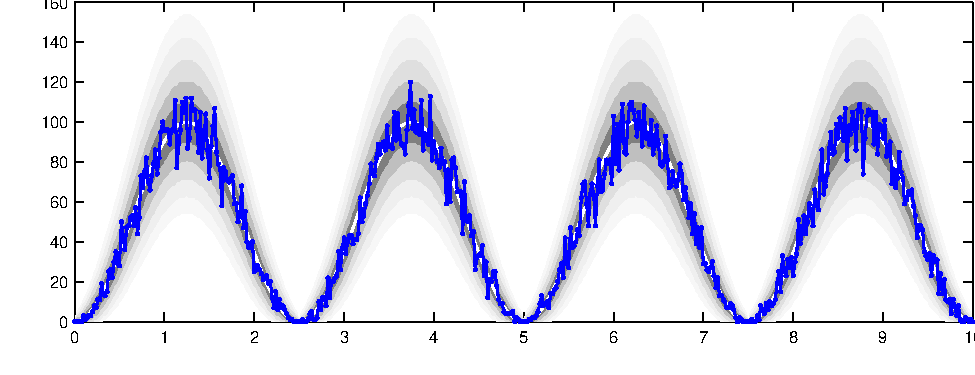
\includegraphics[width=\columnwidth]{figures/cyclostationary-timeseries.pdf}
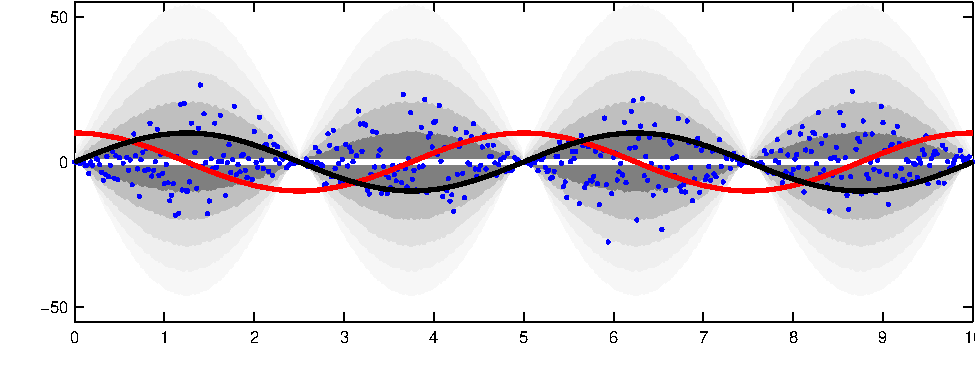
\includegraphics[width=\columnwidth]{figures/cyclostationary-timeseries2.pdf}
\caption[Illustration of cyclo-stationary shot noise]{\label{fig:cyclostationary-shot-noise} \textbf{(a)} Model of
  shot noise in the presence of sinusoidal power modulation, as occurs
  in optical heterodyne detection.  The photodiode sees a power
  modulation at $2f_{mod}$ (white) due to the beat between the upper
  and lower modulation sidebands at $f_{carrier} \pm f_{mod}$.
  The gray levels represent the $1\sigma,\ 2\sigma,
  \cdots, 5\sigma$ ranges for a Poisson distribution.  The blue dots
  are a sample realization of this noise. \textbf{(b)} Subtracting the
  mean from (a) leaves only the noise; its bursty nature is obvious.
  Shown in black and red are the I and Q demodulation waveforms,
  respectively.  It is clear that the in-phase demodulation (I)
  samples regions of the time series with higher variance than the
  quadrature phase (Q).  This leads to a higher variance (shot noise
  level) in the I signal and a lower one in the Q signal relative to
  what one would expect from a na\"ive assumption based on the average
  power considered over a whole period of the waveform.}
\end{figure}
